\documentclass[convert={density=300,size=1080x800,outext=.png}]{standalone}
\usepackage{tikz}
\usetikzlibrary{arrows.meta, arrows}
\begin{document}

%.. tikz:: 
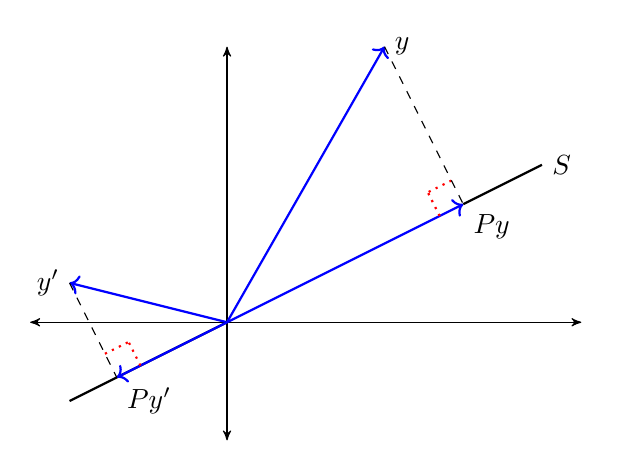
\begin{tikzpicture}
[scale=5, axis/.style={<->, >=stealth'}, important line/.style={thick}, dotted line/.style={dotted, thick,red}, dashed line/.style={dashed, thin}, every node/.style={color=black}] \coordinate(O) at (0,0);
    \coordinate (y') at (-0.4,0.1);
    \coordinate (Py) at (0.6,0.3);
    \coordinate (y) at (0.4,0.7);
    \coordinate (Z1) at (-0.4,-0.2);
    \coordinate (Z2) at (0.8,0.4);
    \coordinate (Py') at (-0.28,-0.14);
    \draw[axis] (-0.5,0)  -- (0.9,0) node(xline)[right] {};
    \draw[axis] (0,-0.3) -- (0,0.7) node(yline)[above] {};
    \draw[important line,blue,thick, ->]  (O) -- (Py) node[anchor = north west, text width=2em] {$P y$};
    \draw[important line,blue, ->]  (O) -- (y') node[left] {$y'$};
    \draw[important line, thick]  (Z1) -- (O) node[right] {};
    \draw[important line, thick]  (Py) -- (Z2) node[right] {$S$};
    \draw[important line, blue,->]  (O) -- (y) node[right] {$y$};
    \draw[important line, blue,->]  (O) -- (Py') node[anchor = north west, text width=5em] {$P y'$};
    \draw[dotted line] (0.54,0.27) -- (0.51,0.33);
    \draw[dotted line] (0.57,0.36) -- (0.51,0.33);
    \draw[dotted line] (-0.22,-0.11) -- (-0.25,-0.05);
    \draw[dotted line] (-0.31,-0.08) -- (-0.25,-0.05);
    \draw[dashed line, black] (y) -- (Py);
    \draw[dashed line, black] (y') -- (Py');
\end{tikzpicture}

\end{document}